% Options for packages loaded elsewhere
\PassOptionsToPackage{unicode}{hyperref}
\PassOptionsToPackage{hyphens}{url}
%
\documentclass[
]{article}
\usepackage{amsmath,amssymb}
\usepackage{iftex}
\ifPDFTeX
  \usepackage[T1]{fontenc}
  \usepackage[utf8]{inputenc}
  \usepackage{textcomp} % provide euro and other symbols
\else % if luatex or xetex
  \usepackage{unicode-math} % this also loads fontspec
  \defaultfontfeatures{Scale=MatchLowercase}
  \defaultfontfeatures[\rmfamily]{Ligatures=TeX,Scale=1}
\fi
\usepackage{lmodern}
\ifPDFTeX\else
  % xetex/luatex font selection
\fi
% Use upquote if available, for straight quotes in verbatim environments
\IfFileExists{upquote.sty}{\usepackage{upquote}}{}
\IfFileExists{microtype.sty}{% use microtype if available
  \usepackage[]{microtype}
  \UseMicrotypeSet[protrusion]{basicmath} % disable protrusion for tt fonts
}{}
\makeatletter
\@ifundefined{KOMAClassName}{% if non-KOMA class
  \IfFileExists{parskip.sty}{%
    \usepackage{parskip}
  }{% else
    \setlength{\parindent}{0pt}
    \setlength{\parskip}{6pt plus 2pt minus 1pt}}
}{% if KOMA class
  \KOMAoptions{parskip=half}}
\makeatother
\usepackage{xcolor}
\usepackage[margin=1in]{geometry}
\usepackage{color}
\usepackage{fancyvrb}
\newcommand{\VerbBar}{|}
\newcommand{\VERB}{\Verb[commandchars=\\\{\}]}
\DefineVerbatimEnvironment{Highlighting}{Verbatim}{commandchars=\\\{\}}
% Add ',fontsize=\small' for more characters per line
\usepackage{framed}
\definecolor{shadecolor}{RGB}{248,248,248}
\newenvironment{Shaded}{\begin{snugshade}}{\end{snugshade}}
\newcommand{\AlertTok}[1]{\textcolor[rgb]{0.94,0.16,0.16}{#1}}
\newcommand{\AnnotationTok}[1]{\textcolor[rgb]{0.56,0.35,0.01}{\textbf{\textit{#1}}}}
\newcommand{\AttributeTok}[1]{\textcolor[rgb]{0.13,0.29,0.53}{#1}}
\newcommand{\BaseNTok}[1]{\textcolor[rgb]{0.00,0.00,0.81}{#1}}
\newcommand{\BuiltInTok}[1]{#1}
\newcommand{\CharTok}[1]{\textcolor[rgb]{0.31,0.60,0.02}{#1}}
\newcommand{\CommentTok}[1]{\textcolor[rgb]{0.56,0.35,0.01}{\textit{#1}}}
\newcommand{\CommentVarTok}[1]{\textcolor[rgb]{0.56,0.35,0.01}{\textbf{\textit{#1}}}}
\newcommand{\ConstantTok}[1]{\textcolor[rgb]{0.56,0.35,0.01}{#1}}
\newcommand{\ControlFlowTok}[1]{\textcolor[rgb]{0.13,0.29,0.53}{\textbf{#1}}}
\newcommand{\DataTypeTok}[1]{\textcolor[rgb]{0.13,0.29,0.53}{#1}}
\newcommand{\DecValTok}[1]{\textcolor[rgb]{0.00,0.00,0.81}{#1}}
\newcommand{\DocumentationTok}[1]{\textcolor[rgb]{0.56,0.35,0.01}{\textbf{\textit{#1}}}}
\newcommand{\ErrorTok}[1]{\textcolor[rgb]{0.64,0.00,0.00}{\textbf{#1}}}
\newcommand{\ExtensionTok}[1]{#1}
\newcommand{\FloatTok}[1]{\textcolor[rgb]{0.00,0.00,0.81}{#1}}
\newcommand{\FunctionTok}[1]{\textcolor[rgb]{0.13,0.29,0.53}{\textbf{#1}}}
\newcommand{\ImportTok}[1]{#1}
\newcommand{\InformationTok}[1]{\textcolor[rgb]{0.56,0.35,0.01}{\textbf{\textit{#1}}}}
\newcommand{\KeywordTok}[1]{\textcolor[rgb]{0.13,0.29,0.53}{\textbf{#1}}}
\newcommand{\NormalTok}[1]{#1}
\newcommand{\OperatorTok}[1]{\textcolor[rgb]{0.81,0.36,0.00}{\textbf{#1}}}
\newcommand{\OtherTok}[1]{\textcolor[rgb]{0.56,0.35,0.01}{#1}}
\newcommand{\PreprocessorTok}[1]{\textcolor[rgb]{0.56,0.35,0.01}{\textit{#1}}}
\newcommand{\RegionMarkerTok}[1]{#1}
\newcommand{\SpecialCharTok}[1]{\textcolor[rgb]{0.81,0.36,0.00}{\textbf{#1}}}
\newcommand{\SpecialStringTok}[1]{\textcolor[rgb]{0.31,0.60,0.02}{#1}}
\newcommand{\StringTok}[1]{\textcolor[rgb]{0.31,0.60,0.02}{#1}}
\newcommand{\VariableTok}[1]{\textcolor[rgb]{0.00,0.00,0.00}{#1}}
\newcommand{\VerbatimStringTok}[1]{\textcolor[rgb]{0.31,0.60,0.02}{#1}}
\newcommand{\WarningTok}[1]{\textcolor[rgb]{0.56,0.35,0.01}{\textbf{\textit{#1}}}}
\usepackage{graphicx}
\makeatletter
\def\maxwidth{\ifdim\Gin@nat@width>\linewidth\linewidth\else\Gin@nat@width\fi}
\def\maxheight{\ifdim\Gin@nat@height>\textheight\textheight\else\Gin@nat@height\fi}
\makeatother
% Scale images if necessary, so that they will not overflow the page
% margins by default, and it is still possible to overwrite the defaults
% using explicit options in \includegraphics[width, height, ...]{}
\setkeys{Gin}{width=\maxwidth,height=\maxheight,keepaspectratio}
% Set default figure placement to htbp
\makeatletter
\def\fps@figure{htbp}
\makeatother
\setlength{\emergencystretch}{3em} % prevent overfull lines
\providecommand{\tightlist}{%
  \setlength{\itemsep}{0pt}\setlength{\parskip}{0pt}}
\setcounter{secnumdepth}{-\maxdimen} % remove section numbering
\ifLuaTeX
  \usepackage{selnolig}  % disable illegal ligatures
\fi
\IfFileExists{bookmark.sty}{\usepackage{bookmark}}{\usepackage{hyperref}}
\IfFileExists{xurl.sty}{\usepackage{xurl}}{} % add URL line breaks if available
\urlstyle{same}
\hypersetup{
  pdftitle={Reinforcement Learning Task 1: Foundation to Q-Values},
  pdfauthor={Student Name},
  hidelinks,
  pdfcreator={LaTeX via pandoc}}

\title{Reinforcement Learning Task 1: Foundation to Q-Values}
\author{Student Name}
\date{2025-06-17}

\begin{document}
\maketitle

{
\setcounter{tocdepth}{2}
\tableofcontents
}
\hypertarget{ex1-markov-chains-conceptual}{%
\section{Ex1: Markov Chains
(Conceptual)}\label{ex1-markov-chains-conceptual}}

\textbf{Markov Property in Financial Markets}

The Markov property assumes future states depend only on the current
state, not the entire history. In financial markets, this translates to:
\emph{P(S\_\{t+1\} \textbar{} S\_t, S\_\{t-1\}, \ldots, S\_0) =
P(S\_\{t+1\} \textbar{} S\_t)}. Our state design captures recent market
momentum through a sliding window, embodying this principle for RL
trading decisions.

\hypertarget{ex2-market-data-preparation}{%
\section{Ex2: Market Data
Preparation}\label{ex2-market-data-preparation}}

\textbf{SPY Data Retrieval and Returns Calculation}

\begin{Shaded}
\begin{Highlighting}[]
\FunctionTok{suppressPackageStartupMessages}\NormalTok{(\{}
  \FunctionTok{library}\NormalTok{(quantmod); }\FunctionTok{library}\NormalTok{(dplyr); }\FunctionTok{library}\NormalTok{(ggplot2)}
  \FunctionTok{library}\NormalTok{(lubridate); }\FunctionTok{library}\NormalTok{(tibble); }\FunctionTok{library}\NormalTok{(moments); }\FunctionTok{library}\NormalTok{(neuralnet)}
\NormalTok{\})}
\FunctionTok{set.seed}\NormalTok{(}\DecValTok{42}\NormalTok{)}
\end{Highlighting}
\end{Shaded}

\begin{Shaded}
\begin{Highlighting}[]
\NormalTok{get\_spy\_data }\OtherTok{\textless{}{-}} \ControlFlowTok{function}\NormalTok{(}\AttributeTok{sd =} \StringTok{"2015{-}01{-}01"}\NormalTok{) \{}
\NormalTok{  spy\_xts }\OtherTok{\textless{}{-}} \FunctionTok{getSymbols}\NormalTok{(}\StringTok{"SPY"}\NormalTok{, }\AttributeTok{src =} \StringTok{"yahoo"}\NormalTok{, }\AttributeTok{from =}\NormalTok{ sd, }\AttributeTok{auto.assign =} \ConstantTok{FALSE}\NormalTok{, }\AttributeTok{warnings =} \ConstantTok{FALSE}\NormalTok{)}
  \FunctionTok{data.frame}\NormalTok{(}\AttributeTok{date =} \FunctionTok{index}\NormalTok{(}\FunctionTok{Ad}\NormalTok{(spy\_xts)), }\AttributeTok{price =} \FunctionTok{as.numeric}\NormalTok{(}\FunctionTok{Ad}\NormalTok{(spy\_xts))) }\SpecialCharTok{\%\textgreater{}\%} 
    \FunctionTok{as\_tibble}\NormalTok{() }\SpecialCharTok{\%\textgreater{}\%} \FunctionTok{arrange}\NormalTok{(date) }\SpecialCharTok{\%\textgreater{}\%} \FunctionTok{filter}\NormalTok{(}\SpecialCharTok{!}\FunctionTok{is.na}\NormalTok{(price))}
\NormalTok{\}}

\NormalTok{calc\_pct\_returns }\OtherTok{\textless{}{-}} \ControlFlowTok{function}\NormalTok{(prices\_df) \{}
\NormalTok{  prices\_df }\SpecialCharTok{\%\textgreater{}\%} \FunctionTok{mutate}\NormalTok{(}\AttributeTok{p\_lag =} \FunctionTok{lag}\NormalTok{(price, }\DecValTok{1}\NormalTok{), }\AttributeTok{ret\_pct =}\NormalTok{ (price }\SpecialCharTok{/}\NormalTok{ p\_lag }\SpecialCharTok{{-}} \DecValTok{1}\NormalTok{) }\SpecialCharTok{*} \DecValTok{100}\NormalTok{) }\SpecialCharTok{\%\textgreater{}\%} 
    \FunctionTok{filter}\NormalTok{(}\SpecialCharTok{!}\FunctionTok{is.na}\NormalTok{(ret\_pct)) }\SpecialCharTok{\%\textgreater{}\%} \FunctionTok{select}\NormalTok{(date, price, ret\_pct)}
\NormalTok{\}}

\NormalTok{spy\_prices }\OtherTok{\textless{}{-}} \FunctionTok{get\_spy\_data}\NormalTok{()}
\NormalTok{spy\_returns }\OtherTok{\textless{}{-}} \FunctionTok{calc\_pct\_returns}\NormalTok{(spy\_prices)}
\FunctionTok{cat}\NormalTok{(}\StringTok{"Data loaded:"}\NormalTok{, }\FunctionTok{nrow}\NormalTok{(spy\_returns), }\StringTok{"observations from"}\NormalTok{, }\FunctionTok{as.character}\NormalTok{(}\FunctionTok{min}\NormalTok{(spy\_returns}\SpecialCharTok{$}\NormalTok{date)), }\StringTok{"to"}\NormalTok{, }\FunctionTok{as.character}\NormalTok{(}\FunctionTok{max}\NormalTok{(spy\_returns}\SpecialCharTok{$}\NormalTok{date)))}
\DocumentationTok{\#\# Data loaded: 2628 observations from 2015{-}01{-}05 to 2025{-}06{-}16}
\end{Highlighting}
\end{Shaded}

\begin{Shaded}
\begin{Highlighting}[]
\FunctionTok{ggplot}\NormalTok{(spy\_returns, }\FunctionTok{aes}\NormalTok{(}\AttributeTok{x =}\NormalTok{ date, }\AttributeTok{y =}\NormalTok{ price)) }\SpecialCharTok{+} \FunctionTok{geom\_line}\NormalTok{(}\AttributeTok{color =} \StringTok{"blue"}\NormalTok{, }\AttributeTok{alpha =} \FloatTok{0.7}\NormalTok{) }\SpecialCharTok{+} 
  \FunctionTok{labs}\NormalTok{(}\AttributeTok{title =} \StringTok{"SPY Price Evolution"}\NormalTok{, }\AttributeTok{x =} \StringTok{""}\NormalTok{, }\AttributeTok{y =} \StringTok{"Price"}\NormalTok{) }\SpecialCharTok{+} \FunctionTok{theme\_minimal}\NormalTok{()}
\end{Highlighting}
\end{Shaded}

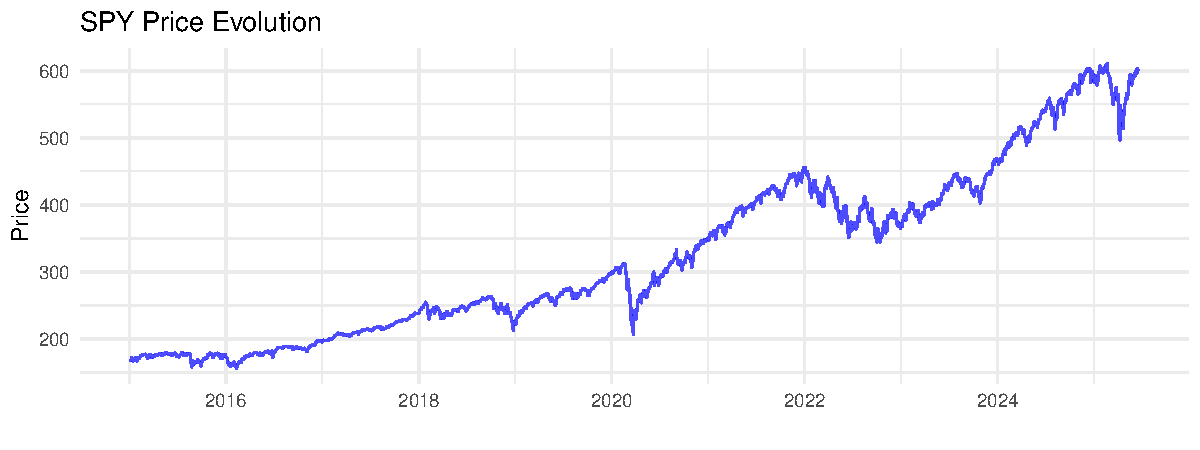
\includegraphics{GroupDTask1_files/figure-latex/data-viz-1.pdf}

\hypertarget{ex3-state-vector-implementation}{%
\section{Ex3: State Vector
Implementation}\label{ex3-state-vector-implementation}}

\textbf{Market State Representation}

\begin{Shaded}
\begin{Highlighting}[]
\NormalTok{INPUT\_NODES }\OtherTok{\textless{}{-}} \DecValTok{10}

\NormalTok{mk\_state\_fct }\OtherTok{\textless{}{-}} \ControlFlowTok{function}\NormalTok{(}\AttributeTok{ws =} \DecValTok{10}\NormalTok{) \{}
  \ControlFlowTok{function}\NormalTok{(ret\_data, t\_idx) \{}
\NormalTok{    s\_vec }\OtherTok{\textless{}{-}}\NormalTok{ ret\_data}\SpecialCharTok{$}\NormalTok{ret\_pct[(t\_idx }\SpecialCharTok{{-}}\NormalTok{ ws }\SpecialCharTok{+} \DecValTok{1}\NormalTok{)}\SpecialCharTok{:}\NormalTok{t\_idx]}
    \FunctionTok{structure}\NormalTok{(}\FunctionTok{list}\NormalTok{(}\AttributeTok{values =}\NormalTok{ s\_vec), }\AttributeTok{class =} \StringTok{"MarketState"}\NormalTok{)}
\NormalTok{  \}}
\NormalTok{\}}
\NormalTok{make\_state }\OtherTok{\textless{}{-}} \FunctionTok{mk\_state\_fct}\NormalTok{(}\AttributeTok{ws =}\NormalTok{ INPUT\_NODES)}

\CommentTok{\# Demonstrate state creation}
\NormalTok{demo\_state }\OtherTok{\textless{}{-}} \FunctionTok{make\_state}\NormalTok{(spy\_returns, }\AttributeTok{t\_idx =} \DecValTok{15}\NormalTok{)}
\FunctionTok{cat}\NormalTok{(}\StringTok{"State vector (10{-}day return window):"}\NormalTok{, }\FunctionTok{round}\NormalTok{(demo\_state}\SpecialCharTok{$}\NormalTok{values, }\DecValTok{3}\NormalTok{))}
\DocumentationTok{\#\# State vector (10{-}day return window): {-}0.783 {-}0.281 {-}0.604 {-}0.916 1.311 0.213 0.505 1.487 {-}0.548 0.234}
\end{Highlighting}
\end{Shaded}

\hypertarget{ex4-q-network-architecture}{%
\section{Ex4: Q-Network Architecture}\label{ex4-q-network-architecture}}

\textbf{Neural Network Q-Value Prediction}

\begin{Shaded}
\begin{Highlighting}[]
\NormalTok{ACTIONS }\OtherTok{\textless{}{-}} \FunctionTok{c}\NormalTok{(}\StringTok{"Buy"}\NormalTok{, }\StringTok{"Sell"}\NormalTok{, }\StringTok{"Hold"}\NormalTok{)}
\NormalTok{NUM\_ACTS }\OtherTok{\textless{}{-}} \FunctionTok{length}\NormalTok{(ACTIONS)}

\NormalTok{nn\_predict\_q }\OtherTok{\textless{}{-}} \ControlFlowTok{function}\NormalTok{(state\_v, }\AttributeTok{model =} \ConstantTok{NULL}\NormalTok{) \{}
  \ControlFlowTok{if}\NormalTok{ (}\FunctionTok{is.null}\NormalTok{(model)) }\FunctionTok{return}\NormalTok{(}\FunctionTok{setNames}\NormalTok{(}\FunctionTok{runif}\NormalTok{(NUM\_ACTS, }\SpecialCharTok{{-}}\DecValTok{1}\NormalTok{, }\DecValTok{1}\NormalTok{), ACTIONS))}
\NormalTok{  input\_mat }\OtherTok{\textless{}{-}} \FunctionTok{matrix}\NormalTok{(state\_v, }\AttributeTok{nrow =} \DecValTok{1}\NormalTok{, }\AttributeTok{byrow =} \ConstantTok{TRUE}\NormalTok{)}
  \FunctionTok{colnames}\NormalTok{(input\_mat) }\OtherTok{\textless{}{-}} \FunctionTok{paste0}\NormalTok{(}\StringTok{"X"}\NormalTok{, }\DecValTok{1}\SpecialCharTok{:}\NormalTok{INPUT\_NODES)}
\NormalTok{  q\_vals }\OtherTok{\textless{}{-}}\NormalTok{ neuralnet}\SpecialCharTok{::}\FunctionTok{compute}\NormalTok{(model, input\_mat)}\SpecialCharTok{$}\NormalTok{net.result}
  \FunctionTok{setNames}\NormalTok{(}\FunctionTok{as.vector}\NormalTok{(q\_vals), ACTIONS)}
\NormalTok{\}}

\CommentTok{\# Demo untrained Q{-}predictions}
\NormalTok{sample\_state }\OtherTok{\textless{}{-}} \FunctionTok{make\_state}\NormalTok{(spy\_returns, }\DecValTok{20}\NormalTok{)}\SpecialCharTok{$}\NormalTok{values}
\NormalTok{demo\_q }\OtherTok{\textless{}{-}} \FunctionTok{nn\_predict\_q}\NormalTok{(sample\_state)}
\FunctionTok{cat}\NormalTok{(}\StringTok{"Sample Q{-}values (untrained):"}\NormalTok{, }\FunctionTok{round}\NormalTok{(demo\_q, }\DecValTok{3}\NormalTok{))}
\DocumentationTok{\#\# Sample Q{-}values (untrained): 0.83 0.874 {-}0.428}
\end{Highlighting}
\end{Shaded}

\hypertarget{ex5-artificial-q-targets}{%
\section{Ex5: Artificial Q-Targets}\label{ex5-artificial-q-targets}}

\textbf{Rule-Based Q-Target Generation}

\begin{Shaded}
\begin{Highlighting}[]
\NormalTok{gen\_art\_q\_target }\OtherTok{\textless{}{-}} \ControlFlowTok{function}\NormalTok{(state\_v, action\_t, reward) \{}
\NormalTok{  q\_t }\OtherTok{\textless{}{-}} \FunctionTok{setNames}\NormalTok{(}\FunctionTok{rep}\NormalTok{(}\DecValTok{0}\NormalTok{, NUM\_ACTS), ACTIONS)}
\NormalTok{  mr\_s }\OtherTok{\textless{}{-}} \FunctionTok{mean}\NormalTok{(state\_v)}
  \ControlFlowTok{if}\NormalTok{ (mr\_s }\SpecialCharTok{\textgreater{}} \FloatTok{0.05}\NormalTok{) \{ q\_t[}\StringTok{"Buy"}\NormalTok{] }\OtherTok{\textless{}{-}} \DecValTok{1}\NormalTok{; q\_t[}\StringTok{"Sell"}\NormalTok{] }\OtherTok{\textless{}{-}} \SpecialCharTok{{-}}\FloatTok{0.5}\NormalTok{; q\_t[}\StringTok{"Hold"}\NormalTok{] }\OtherTok{\textless{}{-}} \FloatTok{0.1}\NormalTok{ \}}
  \ControlFlowTok{else} \ControlFlowTok{if}\NormalTok{ (mr\_s }\SpecialCharTok{\textless{}} \SpecialCharTok{{-}}\FloatTok{0.05}\NormalTok{) \{ q\_t[}\StringTok{"Buy"}\NormalTok{] }\OtherTok{\textless{}{-}} \SpecialCharTok{{-}}\FloatTok{0.5}\NormalTok{; q\_t[}\StringTok{"Sell"}\NormalTok{] }\OtherTok{\textless{}{-}} \DecValTok{1}\NormalTok{; q\_t[}\StringTok{"Hold"}\NormalTok{] }\OtherTok{\textless{}{-}} \FloatTok{0.1}\NormalTok{ \}}
  \ControlFlowTok{else}\NormalTok{ \{ q\_t[}\StringTok{"Buy"}\NormalTok{] }\OtherTok{\textless{}{-}} \FloatTok{0.2}\NormalTok{; q\_t[}\StringTok{"Sell"}\NormalTok{] }\OtherTok{\textless{}{-}} \FloatTok{0.2}\NormalTok{; q\_t[}\StringTok{"Hold"}\NormalTok{] }\OtherTok{\textless{}{-}} \FloatTok{0.5}\NormalTok{ \}}
\NormalTok{  q\_t[action\_t] }\OtherTok{\textless{}{-}}\NormalTok{ q\_t[action\_t] }\SpecialCharTok{+}\NormalTok{ reward}
\NormalTok{  q\_t}
\NormalTok{\}}

\CommentTok{\# Demo artificial targets}
\NormalTok{demo\_targets }\OtherTok{\textless{}{-}} \FunctionTok{gen\_art\_q\_target}\NormalTok{(sample\_state, }\StringTok{"Buy"}\NormalTok{, }\FloatTok{0.5}\NormalTok{)}
\FunctionTok{cat}\NormalTok{(}\StringTok{"Artificial Q{-}targets for \textquotesingle{}Buy\textquotesingle{} action with reward 0.5:"}\NormalTok{, }\FunctionTok{round}\NormalTok{(demo\_targets, }\DecValTok{3}\NormalTok{))}
\DocumentationTok{\#\# Artificial Q{-}targets for \textquotesingle{}Buy\textquotesingle{} action with reward 0.5: 0.7 0.2 0.5}
\end{Highlighting}
\end{Shaded}

\hypertarget{ex6-q-learning-training-loop}{%
\section{Ex6: Q-Learning Training
Loop}\label{ex6-q-learning-training-loop}}

\textbf{Conceptual Training Implementation}

\begin{Shaded}
\begin{Highlighting}[]
\NormalTok{train\_q\_loop\_conceptual }\OtherTok{\textless{}{-}} \ControlFlowTok{function}\NormalTok{(ret\_data, }\AttributeTok{eps =} \DecValTok{2}\NormalTok{, }\AttributeTok{steps =} \DecValTok{50}\NormalTok{, }\AttributeTok{e\_start =} \DecValTok{1}\NormalTok{, }\AttributeTok{e\_end =} \FloatTok{0.1}\NormalTok{, }\AttributeTok{e\_decay =} \FloatTok{0.9}\NormalTok{) \{}
\NormalTok{  curr\_eps }\OtherTok{\textless{}{-}}\NormalTok{ e\_start}
  
  \CommentTok{\# Initialize dummy neural network}
\NormalTok{  dummy\_in }\OtherTok{\textless{}{-}} \FunctionTok{as.data.frame}\NormalTok{(}\FunctionTok{matrix}\NormalTok{(}\FunctionTok{rnorm}\NormalTok{(}\DecValTok{10} \SpecialCharTok{*}\NormalTok{ INPUT\_NODES), }\AttributeTok{ncol =}\NormalTok{ INPUT\_NODES))}
  \FunctionTok{colnames}\NormalTok{(dummy\_in) }\OtherTok{\textless{}{-}} \FunctionTok{paste0}\NormalTok{(}\StringTok{"X"}\NormalTok{, }\DecValTok{1}\SpecialCharTok{:}\NormalTok{INPUT\_NODES)}
\NormalTok{  dummy\_out }\OtherTok{\textless{}{-}} \FunctionTok{as.data.frame}\NormalTok{(}\FunctionTok{matrix}\NormalTok{(}\FunctionTok{rnorm}\NormalTok{(}\DecValTok{10} \SpecialCharTok{*}\NormalTok{ NUM\_ACTS), }\AttributeTok{ncol =}\NormalTok{ NUM\_ACTS))}
  \FunctionTok{colnames}\NormalTok{(dummy\_out) }\OtherTok{\textless{}{-}}\NormalTok{ ACTIONS}
\NormalTok{  dummy\_df }\OtherTok{\textless{}{-}} \FunctionTok{cbind}\NormalTok{(dummy\_in, dummy\_out)}
\NormalTok{  nn\_form }\OtherTok{\textless{}{-}} \FunctionTok{as.formula}\NormalTok{(}\FunctionTok{paste}\NormalTok{(}\FunctionTok{paste}\NormalTok{(ACTIONS, }\AttributeTok{collapse =} \StringTok{" + "}\NormalTok{), }\StringTok{"\textasciitilde{}"}\NormalTok{, }\FunctionTok{paste}\NormalTok{(}\FunctionTok{paste0}\NormalTok{(}\StringTok{"X"}\NormalTok{, }\DecValTok{1}\SpecialCharTok{:}\NormalTok{INPUT\_NODES), }\AttributeTok{collapse =} \StringTok{" + "}\NormalTok{)))}
\NormalTok{  q\_nn\_model }\OtherTok{\textless{}{-}} \FunctionTok{neuralnet}\NormalTok{(nn\_form, }\AttributeTok{data =}\NormalTok{ dummy\_df, }\AttributeTok{hidden =} \FunctionTok{c}\NormalTok{(}\DecValTok{64}\NormalTok{, }\DecValTok{32}\NormalTok{), }\AttributeTok{linear.output =} \ConstantTok{TRUE}\NormalTok{, }\AttributeTok{rep =} \DecValTok{1}\NormalTok{)}
  
  \ControlFlowTok{for}\NormalTok{ (ep\_i }\ControlFlowTok{in} \DecValTok{1}\SpecialCharTok{:}\NormalTok{eps) \{}
\NormalTok{    s\_idx }\OtherTok{\textless{}{-}} \FunctionTok{sample}\NormalTok{(INPUT\_NODES}\SpecialCharTok{:}\NormalTok{(}\FunctionTok{nrow}\NormalTok{(ret\_data) }\SpecialCharTok{{-}}\NormalTok{ steps }\SpecialCharTok{{-}} \DecValTok{1}\NormalTok{), }\DecValTok{1}\NormalTok{)}
    \ControlFlowTok{for}\NormalTok{ (st\_i }\ControlFlowTok{in} \DecValTok{1}\SpecialCharTok{:}\NormalTok{steps) \{}
\NormalTok{      curr\_t }\OtherTok{\textless{}{-}}\NormalTok{ s\_idx }\SpecialCharTok{+}\NormalTok{ st\_i }\SpecialCharTok{{-}} \DecValTok{1}
      \ControlFlowTok{if}\NormalTok{ (curr\_t }\SpecialCharTok{+}\NormalTok{ INPUT\_NODES }\SpecialCharTok{\textgreater{}} \FunctionTok{nrow}\NormalTok{(ret\_data)) }\ControlFlowTok{break}
      
      \CommentTok{\# State normalization}
\NormalTok{      curr\_s\_vec }\OtherTok{\textless{}{-}} \FunctionTok{make\_state}\NormalTok{(ret\_data, curr\_t)}\SpecialCharTok{$}\NormalTok{values}
\NormalTok{      min\_r }\OtherTok{\textless{}{-}} \FunctionTok{min}\NormalTok{(ret\_data}\SpecialCharTok{$}\NormalTok{ret\_pct); max\_r }\OtherTok{\textless{}{-}} \FunctionTok{max}\NormalTok{(ret\_data}\SpecialCharTok{$}\NormalTok{ret\_pct)}
\NormalTok{      norm\_curr\_s }\OtherTok{\textless{}{-}}\NormalTok{ (curr\_s\_vec }\SpecialCharTok{{-}}\NormalTok{ min\_r) }\SpecialCharTok{/}\NormalTok{ (max\_r }\SpecialCharTok{{-}}\NormalTok{ min\_r)}
      \ControlFlowTok{if}\NormalTok{ (}\FunctionTok{is.nan}\NormalTok{(norm\_curr\_s[}\DecValTok{1}\NormalTok{]) }\SpecialCharTok{||}\NormalTok{ (max\_r }\SpecialCharTok{{-}}\NormalTok{ min\_r) }\SpecialCharTok{==} \DecValTok{0}\NormalTok{) norm\_curr\_s }\OtherTok{\textless{}{-}} \FunctionTok{rep}\NormalTok{(}\FloatTok{0.5}\NormalTok{, INPUT\_NODES)}
      
      \CommentTok{\# Action selection (Ex7)}
\NormalTok{      act\_idx }\OtherTok{\textless{}{-}} \FunctionTok{sel\_act\_egreedy}\NormalTok{(nn\_predict\_q, norm\_curr\_s, curr\_eps, q\_nn\_model)}
\NormalTok{      act\_taken }\OtherTok{\textless{}{-}}\NormalTok{ ACTIONS[act\_idx]}
      
      \CommentTok{\# Reward calculation}
\NormalTok{      next\_ret }\OtherTok{\textless{}{-}}\NormalTok{ ret\_data}\SpecialCharTok{$}\NormalTok{ret\_pct[curr\_t }\SpecialCharTok{+} \DecValTok{1}\NormalTok{]}
\NormalTok{      rew }\OtherTok{\textless{}{-}} \ControlFlowTok{if}\NormalTok{ (act\_taken }\SpecialCharTok{==} \StringTok{"Buy"}\NormalTok{) next\_ret }\ControlFlowTok{else} \ControlFlowTok{if}\NormalTok{ (act\_taken }\SpecialCharTok{==} \StringTok{"Sell"}\NormalTok{) }\SpecialCharTok{{-}}\NormalTok{next\_ret }\ControlFlowTok{else} \FloatTok{0.01} \SpecialCharTok{*} \FunctionTok{sign}\NormalTok{(next\_ret)}
\NormalTok{      rew }\OtherTok{\textless{}{-}} \FunctionTok{min}\NormalTok{(}\FunctionTok{max}\NormalTok{(rew, }\SpecialCharTok{{-}}\DecValTok{1}\NormalTok{), }\DecValTok{1}\NormalTok{)}
      
      \CommentTok{\# Q{-}learning update}
\NormalTok{      next\_t }\OtherTok{\textless{}{-}}\NormalTok{ curr\_t }\SpecialCharTok{+} \DecValTok{1}
\NormalTok{      is\_done }\OtherTok{\textless{}{-}}\NormalTok{ (next\_t }\SpecialCharTok{+}\NormalTok{ INPUT\_NODES }\SpecialCharTok{\textgreater{}} \FunctionTok{nrow}\NormalTok{(ret\_data))}
\NormalTok{      norm\_next\_s }\OtherTok{\textless{}{-}} \ControlFlowTok{if}\NormalTok{ (}\SpecialCharTok{!}\NormalTok{is\_done) \{}
\NormalTok{        ns\_vec }\OtherTok{\textless{}{-}} \FunctionTok{make\_state}\NormalTok{(ret\_data, next\_t)}\SpecialCharTok{$}\NormalTok{values}
\NormalTok{        nns }\OtherTok{\textless{}{-}}\NormalTok{ (ns\_vec }\SpecialCharTok{{-}}\NormalTok{ min\_r) }\SpecialCharTok{/}\NormalTok{ (max\_r }\SpecialCharTok{{-}}\NormalTok{ min\_r)}
        \ControlFlowTok{if}\NormalTok{ (}\FunctionTok{is.nan}\NormalTok{(nns[}\DecValTok{1}\NormalTok{]) }\SpecialCharTok{||}\NormalTok{ (max\_r }\SpecialCharTok{{-}}\NormalTok{ min\_r) }\SpecialCharTok{==} \DecValTok{0}\NormalTok{) }\FunctionTok{rep}\NormalTok{(}\FloatTok{0.5}\NormalTok{, INPUT\_NODES) }\ControlFlowTok{else}\NormalTok{ nns}
\NormalTok{      \} }\ControlFlowTok{else} \FunctionTok{rep}\NormalTok{(}\DecValTok{0}\NormalTok{, INPUT\_NODES)}
      
\NormalTok{      max\_q\_next }\OtherTok{\textless{}{-}} \ControlFlowTok{if}\NormalTok{ (}\SpecialCharTok{!}\NormalTok{is\_done) }\FunctionTok{max}\NormalTok{(}\FunctionTok{nn\_predict\_q}\NormalTok{(norm\_next\_s, q\_nn\_model)) }\ControlFlowTok{else} \DecValTok{0}
\NormalTok{      target\_q\_for\_act }\OtherTok{\textless{}{-}}\NormalTok{ rew }\SpecialCharTok{+} \FloatTok{0.95} \SpecialCharTok{*}\NormalTok{ max\_q\_next}
\NormalTok{    \}}
\NormalTok{    curr\_eps }\OtherTok{\textless{}{-}} \FunctionTok{max}\NormalTok{(e\_end, curr\_eps }\SpecialCharTok{*}\NormalTok{ e\_decay)}
\NormalTok{  \}}
  \FunctionTok{invisible}\NormalTok{(q\_nn\_model)}
\NormalTok{\}}
\end{Highlighting}
\end{Shaded}

\hypertarget{ex7-epsilon-greedy-action-selection}{%
\section{Ex7: Epsilon-Greedy Action
Selection}\label{ex7-epsilon-greedy-action-selection}}

\textbf{Exploration vs Exploitation Strategy}

\begin{Shaded}
\begin{Highlighting}[]
\NormalTok{sel\_act\_egreedy }\OtherTok{\textless{}{-}} \ControlFlowTok{function}\NormalTok{(pred\_q\_fn, state\_v, eps, model) \{}
  \ControlFlowTok{if}\NormalTok{ (}\FunctionTok{runif}\NormalTok{(}\DecValTok{1}\NormalTok{) }\SpecialCharTok{\textless{}}\NormalTok{ eps) }\FunctionTok{sample}\NormalTok{(}\DecValTok{1}\SpecialCharTok{:}\NormalTok{NUM\_ACTS, }\DecValTok{1}\NormalTok{)  }\CommentTok{\# Explore: random action}
  \ControlFlowTok{else} \FunctionTok{which.max}\NormalTok{(}\FunctionTok{pred\_q\_fn}\NormalTok{(state\_v, model))   }\CommentTok{\# Exploit: best Q{-}value}
\NormalTok{\}}

\CommentTok{\# Demonstrate epsilon{-}greedy behavior}
\FunctionTok{set.seed}\NormalTok{(}\DecValTok{123}\NormalTok{)}
\NormalTok{demo\_actions }\OtherTok{\textless{}{-}} \FunctionTok{replicate}\NormalTok{(}\DecValTok{10}\NormalTok{, \{}
\NormalTok{  action\_idx }\OtherTok{\textless{}{-}} \FunctionTok{sel\_act\_egreedy}\NormalTok{(nn\_predict\_q, sample\_state, }\AttributeTok{eps =} \FloatTok{0.3}\NormalTok{, }\AttributeTok{model =} \ConstantTok{NULL}\NormalTok{)}
\NormalTok{  ACTIONS[action\_idx]}
\NormalTok{\})}
\FunctionTok{cat}\NormalTok{(}\StringTok{"10 epsilon{-}greedy actions (ε=0.3):"}\NormalTok{, }\FunctionTok{paste}\NormalTok{(demo\_actions, }\AttributeTok{collapse =} \StringTok{", "}\NormalTok{))}
\DocumentationTok{\#\# 10 epsilon{-}greedy actions (ε=0.3): Hold, Sell, Buy, Sell, Hold, Buy, Buy, Buy, Buy, Buy}
\end{Highlighting}
\end{Shaded}


\end{document}
